\chapter{Implementierung}\label{chap:Implementierung}
\thispagestyle{standard}
\pagestyle{standard}
\lfoot{\small Refik Kerimi}

In diesem Kapitel wird die Umsetzung der Applikation beschrieben.

\section{Anforderungsanalyse}\label{sub:Anforderungsanalyse}
Die zu entwickelnde Smart Home Applikation muss das Verhalten einer \acs{PWA} aufweisen. Das heißt es müssen die Attribute aus Kapitel \ref{chap:ProgressiveWebapplikationen} eingebaut werden und danach getestet werden siehe Kapitel \ref{chap:Funktionstest}. Außerdem sollen auch APIs entwickelt werden die es möglich machen mit Services von Drittanbietern die Temperatur zu regeln, mit Hilfe von Geolocation API den Standort zu ermitteln um das Garagentor über GPS automatisch öffnen zu können. Ebenso soll das Steuern der Beleuchtung möglich sein. Diese Applikation soll Offline so weit es geht verwendbar sein. Die Anwendung muss Plattformunabhängig und responsive sein.

\section{Umsetzung der Anforderungen}\label{sub:Umsetzung der Anforderungen}
Zur Umsetzung der Anforderungen aus Kapitel \ref{sub:Anforderungsanalyse} wurden für  User Interfac ReactJS\footnote{https://reactjs.org/docs/getting-started.html} und als CSS Framework Semantic-UI\footnote{https://react.semantic-ui.com/introduction} verwendet. Sematic-UI soll sicherstellen das die Applikation responsives Verhalten aufweist und für alle Bildschirmgrößen geeignet ist. Um die Daten zu versenden, aufzurufen und zu speichern wurde das JSON Key/Value Format, die Fetch API und der Browser Cache verwendet.
Als Browser diente der Google Chrome Version 67.
Die nicht fertigen Funktionen wurden mit Mockups dargestellt, um einen Eindruck zu vermitteln wie die App in Zukunft aussehen soll.

\section{Ausgewählte Programmiersprache und IDE}
Als Programmiersprache wurde \acl{JS} (\acs{JS}) ausgewählt. 
Als Entwicklungsumgebung wurde Webstorm (Version 2018.2) von Jetbrains verwendet. 
Weitere verwendete Tools und Frameworks wurden in Kapitel \ref{sub:Umsetzung der Anforderungen} beschrieben.
\newpage
\section{Ordnerstruktur}
Die zwei wichtigsten Dateien befinden sich wie in Abbildung \ref{fig:OrdnerStrucktur} zu sehen ist, im app Verzeichnis.
Ebenfalls wichtig ist das app.js File das unter \textit{/app/src/js/app.js} zu finden ist.

\begin{figure}[h]
	\centering
	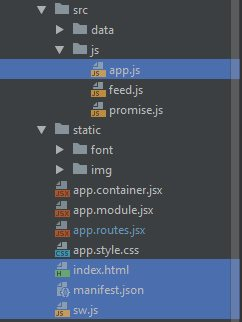
\includegraphics[width=10cm]{BilderAllgemein/Implementierung/OrdnerStrucktur.jpg}\medskip
	\caption{Ordner Strucktur}
	\label{fig:OrdnerStrucktur}
\end{figure} 


\section{Manifest}
Das Manifest wird im Root Folder eingefügt und ist mit der Endung \acs{JSON} deklariert. Der genau Pfad ist \textit{/app/manifest.json}. Wie in Kapitel \ref{sub:Manifest} schon beschrieben wurde, definiert das Manifest File das Aussehen des Icons am Startbildschirm, z.B. den Einstiegspunkt der App und den Namen. 
Die Listing \ref{lst:Manifest.json} zeigt weitere wichtige Eigenschaften:
\newpage
\begin{lstlisting}[language=json, firstnumber=1, caption={Manifest in das Projekt implementieren} {\cite{Manifest}},label=lst:Manifest.json, xleftmargin=50pt]
{
  {
  "name":"PWA Smart Home",
  "short_name":"PWA_SHL_RMJ",
  "start_url":"./",
  "scope":".",
  "display":"standalone",
  "background_color":"#003399",
  "theme_color":"#3F51C5",
  "description":"Keep running with PWA",
  "dir":"ltr",
  "lang":"de-DE",
  "orientation":"portrait-primary",
  "icons":[
    {
      "src":"./static/img/light48.png",
      "type":"image/png",
      "sizes":"48x48"
    },
    {
      "src":"./static/img/light512.png",
      "type":"image/png",
      "sizes":"512x512"
    }
  ]
}
}
\end{lstlisting}

\section{Add to Homescreen}
Damit der Add to Homescreen Banner erscheint müssen die Bedingungen aus dem Kapitel \ref{sub:AddtoHomescreen}erfüllt werden.
Nach Erfüllung dieser Forderungen wird der beforeinstallprompt Event wie in Listing \ref{lst:AddtoHomescreen} aufgerufen und in die deferredPrompt variable gespeichert.

Verzeichnis: \textit{/app/src/js/app.js}

\begin{lstlisting}[language=JavaScript, firstnumber=1, caption={Add to Homescreen Funktion} ,label=lst:AddtoHomescreen, xleftmargin=50pt]
var deferredPrompt;

window.addEventListener('beforeinstallprompt', event => {
    event.preventDefault();
    deferredPrompt = event;
    return false;
});
%\end{lstlisting}

Diese Callbackfunktion wird in die \textit{app.js} Datei implementiert. 

\section{Service Worker und Cache API}
Das Herzstück der Applikation ist der im Kapitel \ref{chap:Basistechnologien} beschriebene Service Worker. Als erstes muss validiert werden ob der Service Worker vom Browser unterstützt wird und danach kann dieser registriert, installiert und aktiviert werden.
In den folgenden Listings \ref{lst:Registrierung}, \ref{lst:Installation} und \ref{lst:Aktivierung} sind die Funktionen, die für den \acs{SW} von Bedeutung sind aufgeführt und die wichtigsten Teile beschrieben.

Verzeichnis: \textit{/app/src/js/app.js}

\begin{lstlisting}[language=JavaScript, firstnumber=1, caption={Registrierung} ,label=lst:Registrierung, xleftmargin=50pt]
//Registrierung und Validierung vom Service Worker
if ('serviceWorker' in navigator) {
    console.log('Service Worker and Notification is supported')
    navigator.serviceWorker.register('/sw.js')
        .then(reg => {
            console.log('Service worker registered!', reg);

        })
        .catch(err => console.log(err));
}
\end{lstlisting}
Die Registriermethode \textit{register()} bekommt als Parameter die Service Worker Datei mitgegeben.

Verzeichnis: \textit{/app/sw.js}

\begin{lstlisting}[language=JavaScript, firstnumber=1, caption={Installation} ,label=lst:Installation, xleftmargin=50pt]
self.addEventListener('install', event => {
    console.log('[Service Worker] Installing Service Worker ....', event);
    event.waitUntil(
        caches.open(cacheName)
            .then(cache => {
                console.log('[Service Worker] Precaching App Frame');
                cache.addAll(filesToCache);
            })
    )
});
}
\end{lstlisting}

Nach dem erneuten Laden der Anwendung wird im Listing \ref{lst:Installation} der Installations Eventlistener aufgerufen. Dieser installiert den Service Worker und cached die angegebenen Dateien um die App offline verwenden zu können. 

Durch die Funktion \textit{waitUntil()} wird mit der Installation gewartet, bis die Dateien die dieser Funktion als Parameter mitgegeben wurden, gecacht wurden. Durch die Cachemethode \textit{cache.All()} werden alle angegeben Dateien aufgerufen und es müssen nicht alle Dateien einzeln eingeben werden.
Nach der Installation wird der Service Worker aktiviert und kann dann vom Browser verwendet werden.

Verzeichnis: \textit{/app/sw.js}

\begin{lstlisting}[language=JavaScript, firstnumber=1, caption={Aktivierung} ,label=lst:Aktivierung, xleftmargin=50pt]
self.addEventListener('activate', event => {
    console.log('[Service Worker] Activating Service Worker ....', event);
    return self.clients.claim();
})
\end{lstlisting}

Durch die \textit{self.clients.claim()} Methode in Zeile 3 wird sichergestellt, dass der Service Worker nur installiert wird wenn alle Bedingungen erfüllt wurden.

Ebenso wichtig ist die fetch-Methode. Diese Methode ruft Daten im Key:Value Format, entweder vom Cache oder falls die Daten nicht im Cache vorhanden sind vom Webserver, auf.

Verzeichnis: \textit{/app/sw.js}

\begin{lstlisting}[language=JavaScript, firstnumber=1, caption={Aktivierung} ,label=lst:fetch, xleftmargin=50pt]
self.addEventListener('fetch', event => {
    event.respondWith(
        caches.match(event.request)
            .then(response => {
                if (response) {
                    return response;
                }else{
                    return fetch(event.request);
                }
            })
    );
});
\end{lstlisting}

In der Callback-Funktion \textit{respondWith()} werden die Daten aufgerufen die match-Methode überprüft ob die Daten sich im Cache befinden.

		
Notizen Video
	Asynchronus Code Abschitt 6 Lektion 62 4:34 
	 

\section{Offline Modus}
Eine der wichtigsten Aufgaben des Caches vom Service Worker ist der Offlinemodus oder das Arbeiten bei schlechter Internetverbindung. Der Cache beinhaltet im Grunde das Index.html File CSS und Bilder oder Icons. Bei der Entwicklung der Anwendung wurden statische Dateien wie im Listing \ref{lst:Cache} verwendet.


\begin{lstlisting}[language=JavaScript, firstnumber=1, caption={Cache} ,label=lst:Cache, xleftmargin=50pt]
let filesToCache = [
    '/',
    '/index.html',
    '/src/js/app.js',
    '/static/img/light48.png',
    '/static/img/dashboard-mockup.jpg',
    '/static/img/bulp.jpeg',
    '/static/img/garage.jpeg',
    '/static/img/Graph_Heizung.JPG',
    '/manifest.json'
];
\end{lstlisting}


\begin{figure}[h]
	\centering
	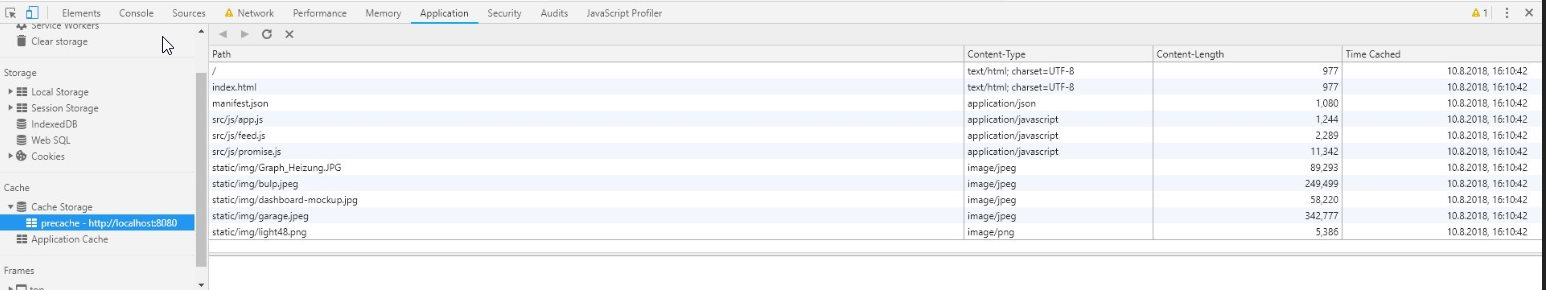
\includegraphics[width=16cm]{BilderAllgemein/Implementierung/Cache.jpg}\medskip
	\caption{Cache}
	\label{fig:Cache}
\end{figure}  

\begin{figure}[h]
	\centering
	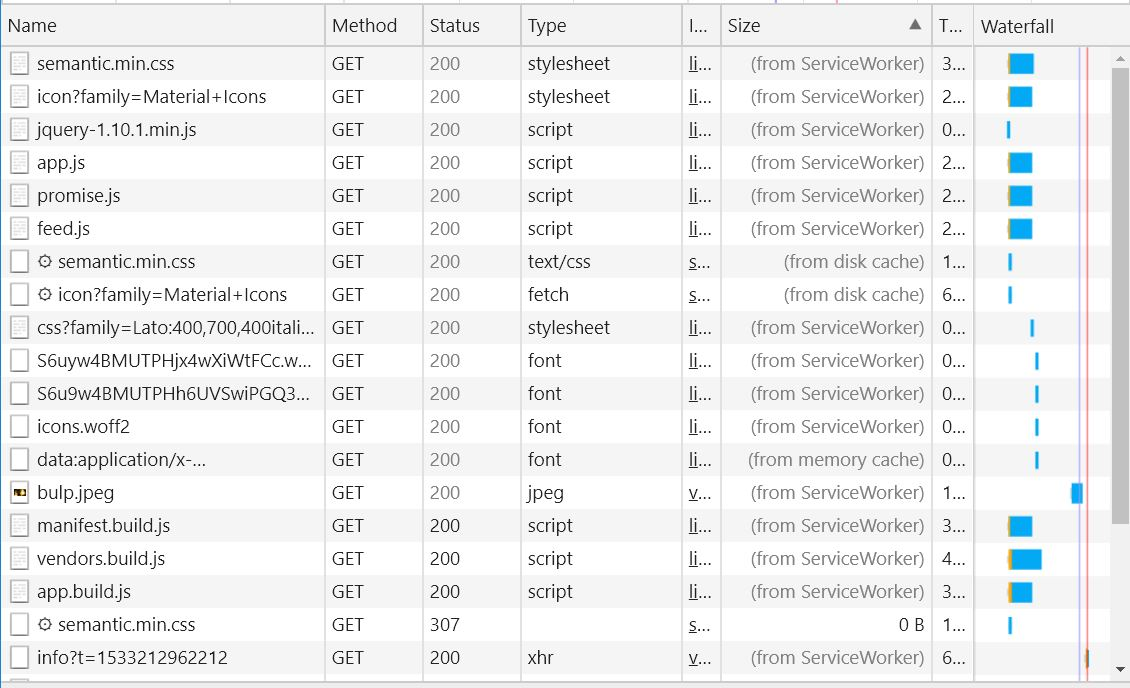
\includegraphics[width=8cm]{BilderAllgemein/Implementierung/aufruf_SW_Browser.jpg}\medskip
	\caption{Datenaufruf Service Worker}
	\label{fig:aufrufSWBrowser}
\end{figure}  

In der Abbildung \ref{fig:aufrufSWBrowser} und \ref{fig:Cache} sind die gecachten Files vom Service Worker im Netzwerk und im Cache zu erkennen.

\begin{figure}[h]
	\centering
	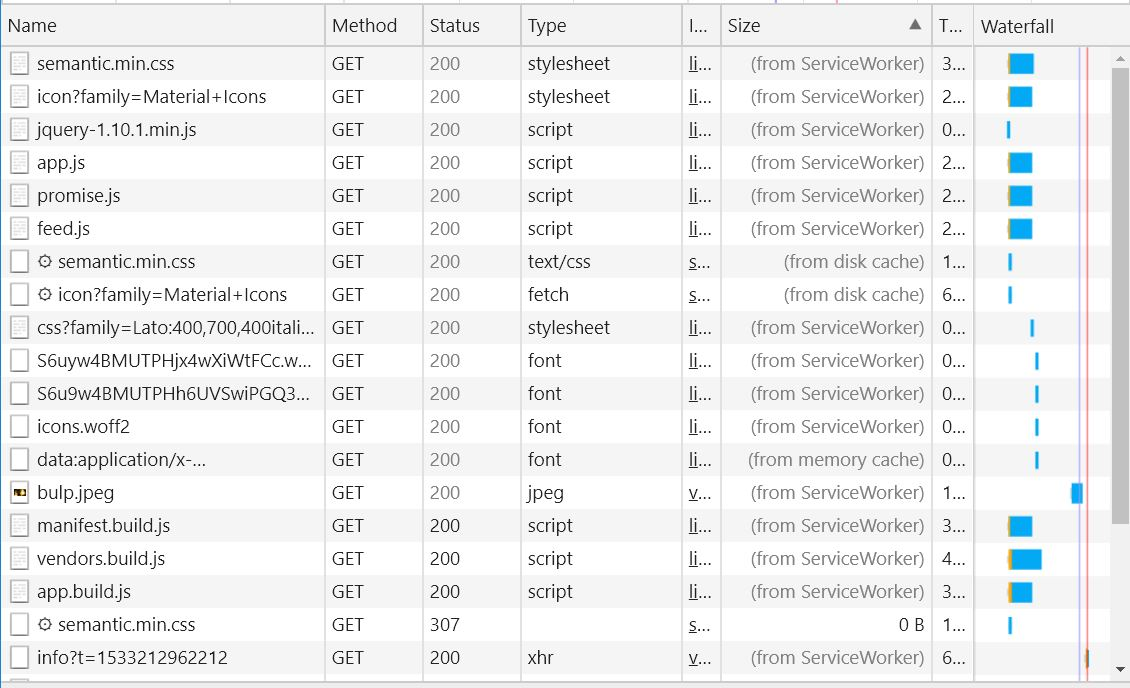
\includegraphics[width=8cm]{BilderAllgemein/Implementierung/aufruf_SW_Browser.jpg}\medskip
	\caption{Datenaufruf Service Worker}
	\label{fig:aufrufSWBrowser}
\end{figure}

\section{Push Notifications}


\section{Geolocation API}











